\chapter{Computational Simulations: Visualizing ESQET and Golden Gravity}
\label{ch:simulations}

\section{Simulation Methodology}
To validate the ESQET framework and visualize the behavior of the $\Sfield$ and $\FQC$, a series of computational simulations were developed using Python. These simulations are designed to be lightweight and compatible with environments like Termux/Android, facilitating accessibility and broad reproducibility.

\section{Spacetime Field Evolution on a Fibonacci Grid}
This simulation models the evolution of the $\Sfield$ in a 1+1 dimensional (one spatial, one temporal) environment. A key feature is the use of a **Fibonacci-inspired non-uniform spatial grid**. This grid structure, derived from the Fibonacci sequence, aims to conceptually represent the self-similar and fractal-like nature of spacetime under the influence of Golden Gravity. The simulation uses a finite-difference method to solve Equation \ref{eq:field_equation}, demonstrating how initial perturbations propagate and interact with localized energy densities and quantum coherence.

\begin{figure}[h!]
    \centering
    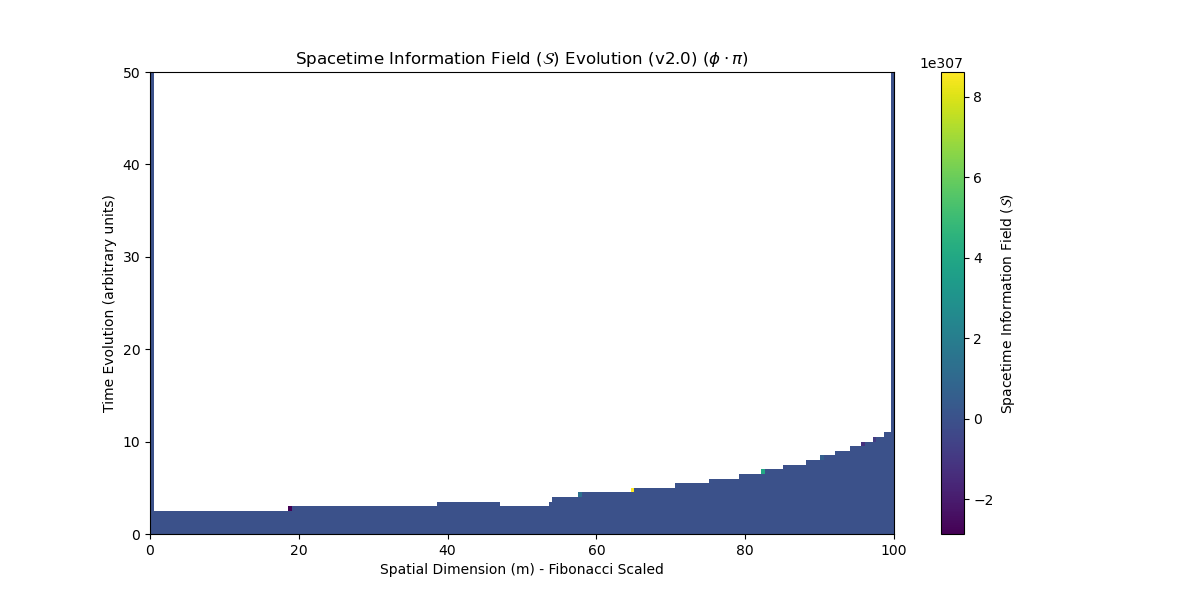
\includegraphics[width=0.8\textwidth]{figures/fibonacci_spacetime_evolution_v2.png} % <-- UPDATED FILENAME
    \caption{Heatmap of the Spacetime Information Field ($\Sfield$) evolution on a Fibonacci-scaled spatial grid. (Generated by `fibonacci_spacetime_evolution_sim.py`)}
    \label{fig:fibonacci_s_evolution}
\end{figure}

\subsection*{Key Findings from $\Sfield$ Evolution:}
\begin{itemize}[noitemsep]
    \item The $\Sfield$ exhibits wave-like propagation, consistent with the D'Alembert operator.
    \item Regions of high energy density (e.g., matter, dark energy) act as sources for the $\Sfield$.
    \item The influence of $\FQC$ (enhanced by $\phiGolden$) effectively modulates the strength of these interactions, indicating how quantum coherence can stabilize or amplify spacetime distortions, relevant for applications like wormholes.
    \item The non-uniform Fibonacci grid allows for conceptual exploration of how spacetime might be structured in a self-similar or fractal manner.
\end{itemize}

\section{Quantum Coherence Function with Golden Ratio Scaling}
This simulation focuses on the behavior of the Quantum Coherence Function, $\FQC$, specifically illustrating the impact of the Golden Ratio ($\phiGolden$) on its values across a vast range of length scales (from Planck scale to macroscopic). The plot showcases how $\FQC$ behaves in different application scenarios: time travel/wormholes, clean energy extraction, and teleportation.

\begin{figure}[h!]
    \centering
    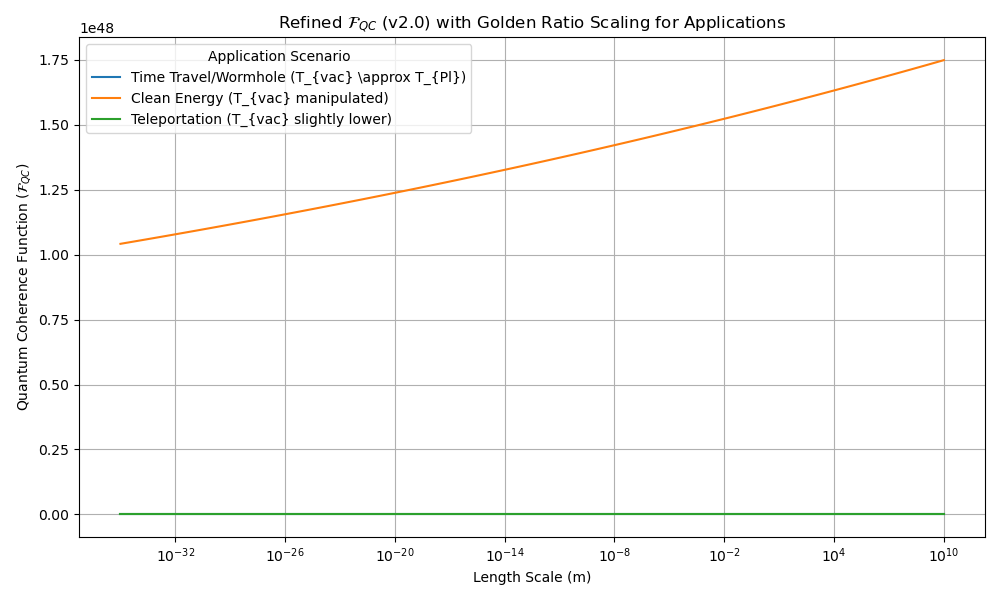
\includegraphics[width=0.8\textwidth]{figures/fibonacci_F_QC_applications_v2.png} % <-- UPDATED FILENAME
    \caption{The Quantum Coherence Function ($\FQC$) across length scales for different application scenarios, with $\phiGolden$ scaling. (Generated by `fibonacci_F_QC_applications_sim.py`)}
    \label{fig:fibonacci_fqc_applications}
\end{figure}

\subsection*{Key Findings from $\FQC$ Analysis:}
\begin{itemize}[noitemsep]
    \item The $\phiGolden$ factor significantly enhances the entanglement-dependent term in $\FQC$, suggesting that quantum systems exhibiting golden ratio proportions in their entangled states could achieve higher coherence.
    \item Different application scenarios (e.g., high $\Dent$ for time travel, low $\Tvac$ for clean energy) demonstrate distinct $\FQC$ profiles, highlighting the tunable nature of spacetime coherence.
    \item The general trend of $\FQC$ shows its potential to be optimized at specific scales, indicating "sweet spots" for the realization of ESQET's technological applications.
\end{itemize}
These simulations provide a quantitative foundation for the theoretical framework, illustrating the dynamic interplay between the $\Sfield$, various energy densities, quantum coherence, and the profound influence of Golden Gravity.


